\documentclass[conference]{IEEEtran}
\IEEEoverridecommandlockouts
% The preceding line is only needed to identify funding in the first footnote. If that is unneeded, please comment it out.
%Template version as of 6/27/2024
\usepackage{float} 
% \usepackage{hyperref}
\usepackage[
backend=biber,
style=authoryear,
natbib=true,
maxbibnames=99,
maxcitenames=1,
mincitenames=1,
url=false,
doi=false,
isbn=false,
eprint=true
]{biblatex}

\DeclareSourcemap{
  \maps[datatype=bibtex]{
    \map{
      \step[fieldsource=archiveprefix, match=\regexp{arXiv}]
      \step[fieldset=eprinttype, fieldvalue={arxiv}]
    }
  }
}

\DeclareFieldFormat{eprint:arxiv}{arXiv preprint arXiv\addcolon\space #1}

\addbibresource{refs.bib}

\DeclareCiteCommand{\citet}
  {}
  {\printtext[bibhyperref]{%
     \printnames{labelname}%
     \setunit{\addspace}%
     \printlabeldateextra}}
  {\multicitedelim}
  {}

\DeclareCiteCommand{\citep}
  {\bibopenparen}
  {\printtext[bibhyperref]{%
     \printnames{labelname}%
     \setunit{\addspace}%
     \printlabeldateextra}}
  {\multicitedelim}
  {\bibcloseparen}


\usepackage[colorlinks,citecolor=blue,linkcolor=blue,bookmarks=false,hypertexnames=true, urlcolor=blue]{hyperref} 
\usepackage{amsmath,amssymb,amsfonts}
\usepackage{algorithmic}
\usepackage{graphicx}
\usepackage{textcomp}
\def\BibTeX{{\rm B\kern-.05em{\sc i\kern-.025em b}\kern-.08em
    T\kern-.1667em\lower.7ex\hbox{E}\kern-.125emX}}
\begin{document}

\title{Where do Gradient Methods Really Happen? Maybe Not Where We Expected\\
\thanks{*Equal contribution }
}

\author{\IEEEauthorblockN{Artur Babayan\textsuperscript{*}}
\IEEEauthorblockA{\textit{HSE University} \\
Moscow, Russia}
\and
\IEEEauthorblockN{Nikita Musalov\textsuperscript{*}}
\IEEEauthorblockA{\textit{HSE University} \\
Moscow, Russia}
\and
\IEEEauthorblockN{Maksim Kopnev\textsuperscript{*}}
\IEEEauthorblockA{\textit{HSE University} \\
Moscow, Russia}
\and
\IEEEauthorblockN{Aleksey Sivolotskiy\textsuperscript{*}}
\IEEEauthorblockA{\textit{HSE University} \\
Moscow, Russia}
\and
\IEEEauthorblockN{Sergey Samsonov}
\IEEEauthorblockA{\textit{HSE University} \\
Moscow, Russia}
}

\maketitle

\begin{abstract}
We study the paper \citet{SongDoesSGD}, which examines the hypothesis that neural network training takes place in low-dimensional subspaces. The authors show that the observed alignment of the gradient with a dominant subspace does not necessarily imply that the principal learning dynamics occur within that subspace.

Within the scope of this project, we first plan to reproduce the main results of the paper for the toy model, MLP, CNN, and Transformer settings. We then intend to extend the study by considering alternative optimizers, other low-dimensional subspaces, and the effect of architectural properties of neural networks on the observed phenomenon.
\end{abstract} 

\section{Introduction}

In modern deep learning, model parameter spaces are high-dimensional; however, recent studies show that effects associated with low-dimensional spaces are observed during training \citep{GurAriGD, SongDoesSGD, LiDLDR}. In the works \citep{GurAriGD, SongDoesSGD} the authors study a phenomenon in which, in a k-class classification problem, the gradient aligns with the dominant subspace after several training steps. The hypothesis that all learning takes place in this subspace was refuted in \citet{SongDoesSGD}. The problem of identifying a low-dimensional subspace in which training can be performed is also considered in other lines of work, which are discussed in more detail in the literature review.

The goal of this work is to examine the gradient alignment phenomenon across a broader range of optimizers, such as Muon, forward-gradient methods, among others, as well as across different low-dimensional subspaces. In addition, we aim to provide a theoretical justification for some of the empirically obtained results.

\section{Related work}

The scientific landscape surrounding this topic naturally falls into several lines of work.

The first and most closely related line consists of works on the Hessian spectrum and on the alignment of the gradient with its top eigenspace. Early studies \citep{sagun2017eigenvalueshessiandeeplearning, sagun2018empiricalanalysishessianoverparametrized, ghorbani2019},already showed that the Hessian spectrum in deep networks typically has a pronounced structure: a bulk concentrated near zero and a small number of outlier eigenvalues. Against this background, the work \citet{GurAriGD} formulated a strong hypothesis: after a short initial phase, the gradient aligns with a small subspace spanned by several top Hessian eigenvectors. A more recent theoretical work \citet{ArousHighDimensional} showed, using simplified high-dimensional mixture models, that a similar alignment can arise in a mathematically rigorous way. However, it was precisely the paper \citet{SongDoesSGD} that provided a fundamental counterexample to a direct interpretation of this observation: when projecting the update onto the dominant Hessian subspace, training stops; in some cases, the loss even starts to increase, while the bulk component of the update remains surprisingly effective.

The latter paper provides the most important reference results for our project. First, it formalizes the dominant subspace as the span of the top-k Hessian eigenvectors, where the standard choice of k is the number of classes in the classification task. Second, it shows that for SGD in the gradient-flow regime, spurious alignment is caused primarily by stochastic noise, whereas for GD at the Edge of Stability, similar alignment is related to a self-stabilization mechanism. Third, in Appendix F, it demonstrates the same negative effect for SGDM and Adam. This led us to the next step: to determine to what extent this negative result depends on the choice of optimizer and on the way the subspace is defined.

The second line of literature concerns the more general idea that neural network problems have low effective dimensionality. The simplest formulation appears in \citet{LiMeasuring}: the network is trained not in the full parameter space, but in a fixed random subspace, and the minimal sufficient dimension is used as a measure of task complexity. In parallel, a stronger empirical hypothesis was proposed in \citet{LiDLDR}, where the DLDR method was introduced and it was shown that some networks can be effectively trained in spaces with dimensions on the order of tens. These works clearly show that a negative result for one specific subspace does not close the topic of low-dimensional training as a whole.

Several related papers also belong to this line of work. In NLP \citet{ZhangFineTuning} shows that fine-tuning pretrained language models can be interpreted through small task-specific subspaces. In few-shot learning, \citet{GauchFewShot} proposes SubGD, an approach based on the eigendecomposition of the autocorrelation matrix of update directions. These works clearly indicate that, as an alternative to the Hessian top-k subspace, one can consider subspaces constructed not from curvature, but from the statistics of gradients or updates themselves.

\section{Problem}

Let
\[
L(\theta) = \frac{1}{n}\sum_{i=1}^n l_i(\theta)
\]
be the empirical loss function, let $\theta_t$ denote the model parameters at step $t$, let $g_t$ be either a stochastic or full gradient, and let
\[
u_t = \mathcal{O}_t(g_t,s_t)
\]
be the "raw" update vector produced by the optimizer $\mathcal{O}$ with internal state $s_t$. For the Hessian
\[
H_t = \nabla^2 L(\theta_t)
\]
we denote by $S_{t,k}^H$ the subspace spanned by the top-k eigenvectors of $H_t$, and by $P_{t,k}^H$ the orthogonal projector onto this subspace. This is precisely the dominant subspace in the sense of the original paper.

Similarly, we introduce several alternative families of subspaces. 
The subspace $S_{t,k}^C$ is the top-$k$ eigenspace of the gradient covariance matrix $C_t$, and $S_{t,k}^R$ is a random $k$-dimensional subspace.

We also consider optimizer-induced subspaces. For optimizers with momentum, let $m_t$ denote the momentum vector or the first-moment estimate. We define $S_{t,k}^M$ as the top-$k$ eigenspace of the covariance matrix of recent momentum vectors. This subspace is intended to capture the main directions accumulated by the optimizer dynamics rather than by the Hessian geometry.

For adaptive optimizers, let $a_t \in \mathbb{R}^p$ denote the vector of coordinate-wise effective learning rates, for example
\[
a_t = \frac{1}{\sqrt{v_t} + \varepsilon}
\]
for Adam-type methods. We define $S_{t,k}^A$ as the coordinate subspace spanned by the $k$ coordinates with the largest adaptive learning rates. This subspace captures directions that are explicitly amplified by the adaptive preconditioner.

Finally,
\[
S_{t,k}^{\text{St}} = \operatorname{span}(Q_t)
\]
is a learnable subspace defined by an orthonormal basis $Q_t \in \operatorname{St}(k,p)$ on the Stiefel manifold.

For each family of subspaces $U$ and each optimizer $\mathcal{O}$, we consider three trajectories:
\[
\theta_{t+1}^{\text{full}} = \theta_t - \eta_t u_t, 
\]
\[
\quad \theta_{t+1}^{U} = \theta_t - \eta_t P_{U_t}u_t,, \quad \theta_{t+1}^{{U^\bot}} = \theta_t - \eta_t (I-P_{U_t})u_t,
\]


\section{Quality metrics}

In this paper, we plan to investigate the behavior of optimizers by projecting their updates onto low-dimensional subspaces, which naturally leads to the following metrics:

\textbf{Alignment}
\[
\chi_S(v) = \frac{\|P_S v\|}{\|v\|}
\]
This metric shows what proportion of the vector lies within the selected subspace.

In addition to the instantaneous alignment value, we use an exponential moving average (EMA) of the alignment score:
\[
\overline{\chi}_{S,t}
=
\beta \overline{\chi}_{S,t-1}
+
(1-\beta)\chi_S(v_t).
\]
Following the protocol of \citet{SongDoesSGD}, the projection phase starts once the EMA of the alignment score exceeds the threshold $0.95$. In our experiments, this switching rule determines the first step from which we replace the full optimizer update by either the projected update $P_{S_t}u_t$ or the orthogonal projected update $(I-P_{S_t})u_t$.

\textbf{Loss/Accuracy} 

As task-level metrics, we report training loss, validation loss, and accuracy. These metrics are used to test whether high alignment with a subspace corresponds to actual learning progress, since a subspace may explain most of the gradient norm while still failing to decrease the loss or improve predictive quality.

\textbf{Projected descent ratio}

Alignment alone does not show whether a subspace is useful for optimization. 
Therefore, we also measure how much of the predicted one-step loss decrease is preserved after projecting the optimizer update onto a subspace.

Using the second-order Taylor approximation,
\[
L(\theta-\eta u)
\approx
L(\theta)
-
\eta \langle g, u\rangle
+
\frac{\eta^2}{2}u^\top H u,
\]
where \(g=\nabla L(\theta)\), \(H=\nabla^2L(\theta)\), and \(u\) is the update direction produced by the optimizer.

For a subspace \(S\) with projector \(P_S\), the projected update is
\[
u_S = P_S u.
\]
We define the projected descent ratio as
\[
\rho_S
=
\frac{
\eta \langle g, P_Su\rangle
-
\frac{\eta^2}{2}(P_Su)^\top H(P_Su)
}{
\eta \langle g, u\rangle
-
\frac{\eta^2}{2}u^\top H u
}.
\]

This metric compares the predicted loss decrease of the projected update with the predicted loss decrease of the original full update.

The interpretation is as follows:
\begin{itemize}
    \item \(\rho_S \approx 1\): the projected update preserves almost all useful loss decrease of the full update, so the subspace is useful for optimization;
    \item \(0 < \rho_S < 1\): the projected update decreases the loss, but less effectively than the full update;
    \item \(\rho_S \approx 0\): the projected update provides almost no useful progress;
    \item \(\rho_S < 0\): the projected update is predicted to increase the loss, so the subspace is harmful for optimization;
    \item \(\rho_S > 1\): the projected update is predicted to decrease the loss even more than the full update.
\end{itemize}

In our experiments, a subspace is considered useful only if it has a high projected descent ratio and this is confirmed by the actual training loss and validation accuracy. Thus, high alignment \(\chi_S(u)\) is not sufficient by itself: a subspace may explain most of the update norm but still fail to produce meaningful loss decrease.

\section{Research questions}

The main question of the project is whether the conclusion of \citet{SongDoesSGD} depends on the choice of optimizer and on the way the low-dimensional subspace is defined.

More specifically, we study the following questions:

\begin{enumerate}
    \item Does the failure of dominant-subspace training persist for optimizers whose update geometry differs substantially from SGD, such as AdamW, Muon, forward-gradient method, and zero-order methods?
    
    \item Do alternative low-dimensional subspaces, such as gradient-covariance subspaces, random subspaces, or learnable subspaces, preserve more useful training progress than the top Hessian eigenspace?
    
    \item Is high alignment between an update direction and a subspace predictive of actual loss decrease, or can it remain a spurious indicator across different optimizers and architectures?
    
    \item Can the observed behavior be explained through simple geometric quantities such as dominant/bulk effective learning rates, noise level, or curvature anisotropy?
\end{enumerate}


\section{Plan}
We divide the project into a mandatory part and a set of optional extensions.
\subsection{Mandatory part}
\begin{enumerate}
    \item \textbf{Reproduction of the main experiments.}
    
    We first reproduce the main results of \citet{SongDoesSGD} on the neural network settings considered in the paper: MLP on MNIST-5k, CNN on CIFAR10-5k, and Transformer on SST2-1k.
    
    The goal of this stage is to verify that our code reproduces the key phenomenon: Dom-SGD stops decreasing the loss, while Bulk-SGD remains close to the original SGD trajectory.
    \item \textbf{Implementation of a unified projection framework.}
    
    We implement a common interface that allows us to take an update vector produced by an arbitrary optimizer and project it either onto a chosen subspace \(U_t\) or onto its orthogonal complement \(U_t^\perp\). 
    
    This stage is necessary to compare different optimizers under the same experimental protocol.
    \item \textbf{Experiments with additional optimizers.}
    
    We extend the projection experiments to optimizers whose update directions differ from SGD. The mandatory set includes Adam, AdamW and Muon. If computationally feasible, we also include forward-gradient methods, and zero-order methods.
    
    For each optimizer, we compare the full update, the projected update, and the orthogonal projected update.
    \item \textbf{Evaluation and metrics.}
    
    For every experiment, we report training loss, validation accuracy and alignment score \(\chi_S(u_t)\). These metrics allow us to distinguish between geometric alignment and actual learning progress.
    \item \textbf{Analysis of results.}
    
    We analyze whether the conclusion of \citet{SongDoesSGD} remains valid for the tested optimizers and whether any optimizer produces a qualitatively different behavior.

    \item \textbf{Alternative low-dimensional subspaces.}
    
    We test whether subspaces not defined by the top Hessian eigenvectors are more useful for projected training. In particular, we consider random subspaces, gradient-covariance subspaces, momentum-induced top-$k$ subspaces, adaptive learning-rate top-$k$ subspaces, and, if feasible, learnable subspaces.
\end{enumerate}
\subsection{Optional extensions}
\begin{enumerate}
    \item \textbf{Larger language-model experiment.}
    
    If the mandatory experiments are completed successfully, we test the same phenomenon on a small GPT-like model such as NanoGPT. This experiment is treated as optional because it is computationally more expensive.

    \item \textbf{Reproduction of experiments on VGG11 and ResNet8 architectures.}

    We reproduce the main experiments of \citet{SongDoesSGD} on two additional architectures: VGG11 and ResNet8 on CIFAR10-5k
    
    \item \textbf{Simplified theoretical explanation.}
    
    We attempt to formulate a qualitative explanation of the observed effects using simple models of anisotropic curvature, optimizer-induced update geometry, and noise. This part is exploratory and is not required for the main empirical contribution of the project.
\end{enumerate}

\section{Outcomes}

\begin{enumerate}
    \item Open JAX/PyTorch implementation of all conducted experiments
    \item A set of reproducible plots
    \item New experiments
    \begin{enumerate}
        \item Other optimizers will be considered
        \item Projections will be performed onto other low-dimensional subspaces
        \item The experiment will be conducted for a language model
    \end{enumerate}
    \item A theoretical explanation of the observed effects
\end{enumerate}


\section{Current results}

At the current stage of the project, we have implemented the main experimental infrastructure and a significant part of the planned experiments.

First, we implemented all neural network architectures considered in \citet{SongDoesSGD}:
\begin{enumerate}
    \item 3-layer MLP with a width of 200 and tanh activation functions;
    \item 3-layer CNN with a width of 32 and ReLU activation functions;
    \item 2-layer Transformer with a hidden dimension of 64 and 8 attention
heads;
    \item VGG11;
    \item ResNet8.
\end{enumerate}
Second, we prepared the following datasets used in \citet{SongDoesSGD}:
\begin{enumerate}
    \item MNIST-5k: a subset of 5\,000 training samples from the MNIST dataset;
    \item CIFAR10-5k: a subset of 5\,000 training samples from the CIFAR-10 dataset;
    \item SST2-1k: a subset of 1\,000 training samples from the SST-2 dataset.
\end{enumerate}

Third, we added support for a broader set of optimizers. In addition to the optimizers considered in the original paper, our implementation currently supports:
\begin{enumerate}
    \item SGD;
    \item SGD with momentum;
    \item Adam;
    \item AdamW;
    \item Muon;
    \item forward-gradient methods;
    \item MeZO;
    \item SubZero.
\end{enumerate}

Fourth, we implemented the projection mechanism for different types of low-dimensional subspaces. At the current stage, the following projectors are available:
\begin{enumerate}
    \item projection onto the top-$k$ Hessian eigenspace;
    \item projection onto a random low-dimensional subspace.
\end{enumerate}

Finally, we developed a unified experimental runner. It allows us to run the same experimental protocol for an arbitrary combination of architecture, optimizer, and projector. This makes it possible to compare full updates, projected updates, and orthogonal projected updates in a consistent way across different experimental settings.

\subsection{Preliminary experiments}

After implementing the main experimental infrastructure, we conducted several preliminary experiments to verify the correctness of the code and reproduce the key effects from \citet{SongDoesSGD}.

\paragraph{Smoke test on a toy problem}

At the first stage, we tested our implementation on a simple toy binary classification problem. For this experiment, we used a small model with approximately 300 parameters. The goal of this experiment was not to obtain a final result, but to check that different optimizers and projectors can be run within a unified protocol and produce meaningful behavior.

In this experiment, we compared several update variants:
\begin{enumerate}
    \item the standard update without projection;
    \item projection onto a random subspace;
    \item projection onto the orthogonal complement of a random subspace;
    \item projection onto the top-$k$ Hessian subspace;
    \item projection onto the orthogonal complement of the top-$k$ Hessian subspace.
\end{enumerate}

\begin{figure}[H]
    \centering
    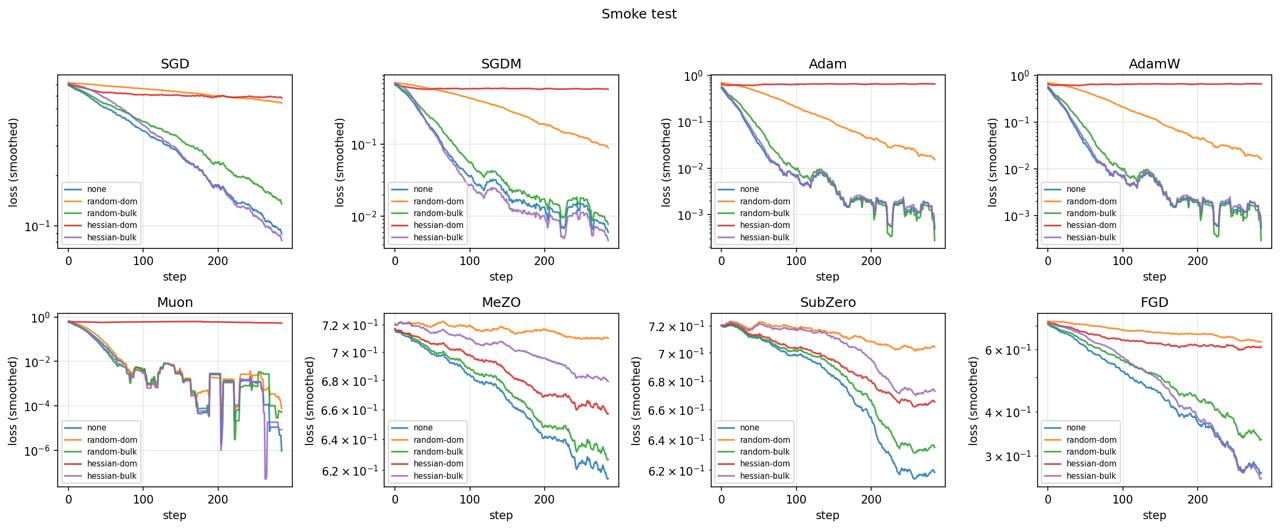
\includegraphics[width=1\linewidth]{smoke_test.png}
    \caption{
    Smoke test on a toy binary classification problem with a small model of about 300 parameters.
    The experiment compares full updates, random-subspace projections, Hessian top-$k$ projections, and their orthogonal complements for several optimizers.
    }
    \label{fig:placeholder}
\end{figure}

\paragraph{Low-rank structure of the Hessian}

Before running the projection experiments, we also checked whether the Hessian in our implementation has the same low-rank structure as reported in \citet{SongDoesSGD}. For this purpose, we tracked the top-30 eigenvalues of the training loss Hessian during SGD training of the MLP model on MNIST-5k.

The obtained plot shows a clear separation between the first 10 eigenvalues and the remaining ones. This is consistent with the fact that MNIST is a 10-class classification problem, so the dominant Hessian subspace is expected to have dimension \(k=10\). The remaining eigenvalues are substantially smaller and form the bulk part of the spectrum. Thus, this experiment confirms that our setup reproduces the spectral structure needed for the dominant/bulk subspace analysis.

\begin{figure}
    \centering
    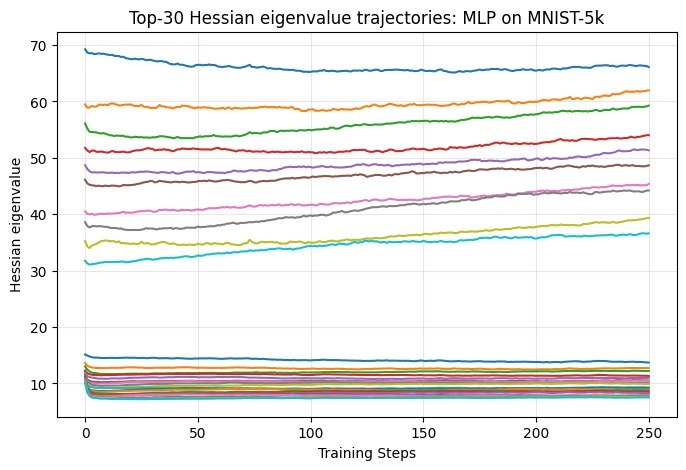
\includegraphics[width=1\linewidth]{mlp_mnist_hessian.png}
    \caption{
    Top-30 Hessian eigenvalue trajectories for MLP on MNIST-5k.
    The first 10 eigenvalues are clearly separated from the remaining part of the spectrum, which supports the low-rank Hessian structure observed in \citet{SongDoesSGD}.
    }
    \label{fig:placeholder}
\end{figure}

\paragraph{Reproduction of the MLP on MNIST-5k experiment for SGD}

Next, we reproduced one of the basic experiments from \citet{SongDoesSGD}: training a 3-layer MLP on MNIST-5k with the SGD optimizer. Before the switching point, the model is trained with standard SGD. After that, we compare two trajectories: projection of the update onto the dominant subspace and projection onto the bulk subspace.

The obtained result qualitatively matches the result of the original paper. After switching to the dominant projection, the loss stops decreasing and even starts to grow gradually. At the same time, the bulk projection continues to decrease the loss. This confirms that the top-$k$ Hessian subspace, despite having a high alignment value, is not a useful subspace for further training in this experiment.

\begin{figure}[H]
    \centering
    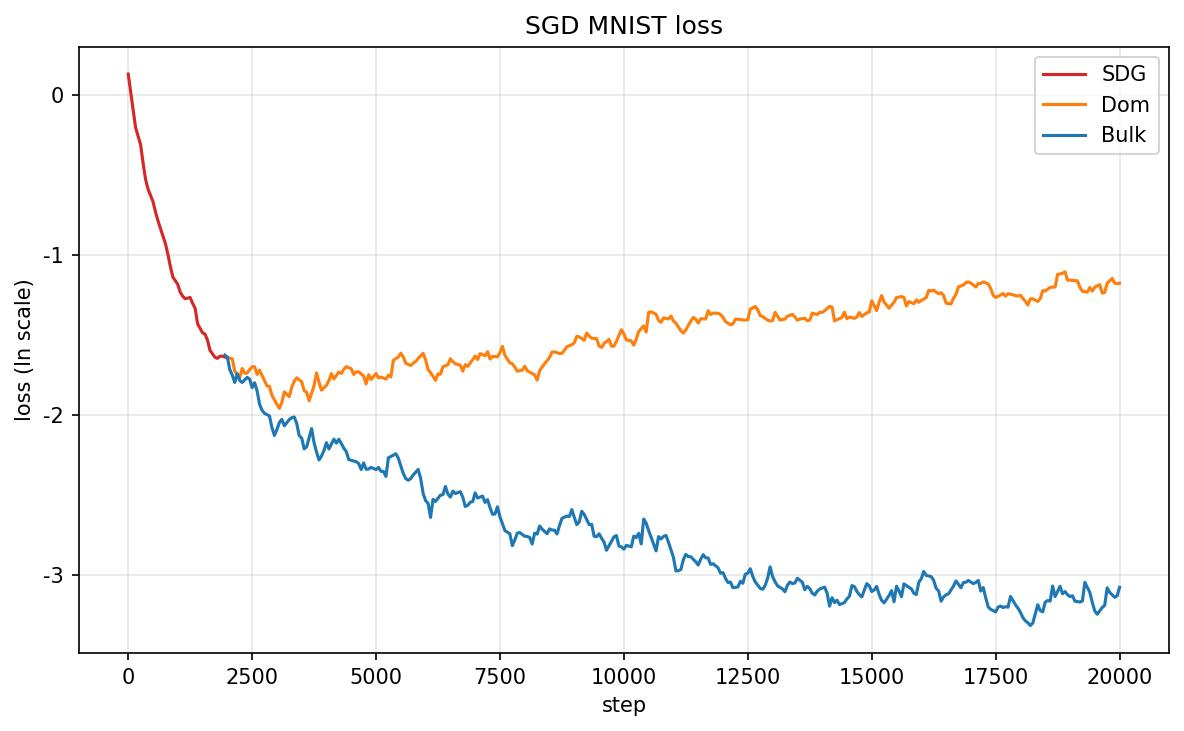
\includegraphics[width=1\linewidth]{sgd_mnist.png}
    \caption{
    Reproduction of the MLP on MNIST-5k experiment with SGD.
    The orange curve corresponds to training after projecting the update onto the dominant Hessian subspace, while the blue curve corresponds to projection onto the bulk subspace.
    Dominant-subspace training stops decreasing the loss, whereas bulk-subspace training continues to make progress.
    }
    \label{fig:placeholder}
\end{figure}

\paragraph{Reproduction of the MLP on MNIST-5k experiment for SGDM}

An analogous experiment was conducted for SGD with momentum. This case is especially important because momentum changes the geometry of the update vector compared to standard SGD: the update direction depends not only on the current gradient, but also on the accumulated history of previous gradients.

Nevertheless, the observed behavior remains similar. After projection onto the dominant Hessian subspace, training does not continue: the loss starts to increase. At the same time, the bulk projection preserves the ability to decrease the loss. This shows that even for an optimizer with momentum, the useful part of the update in this experiment lies mostly not in the top-$k$ Hessian subspace, but in its orthogonal complement.

\begin{figure}[H]
    \centering
    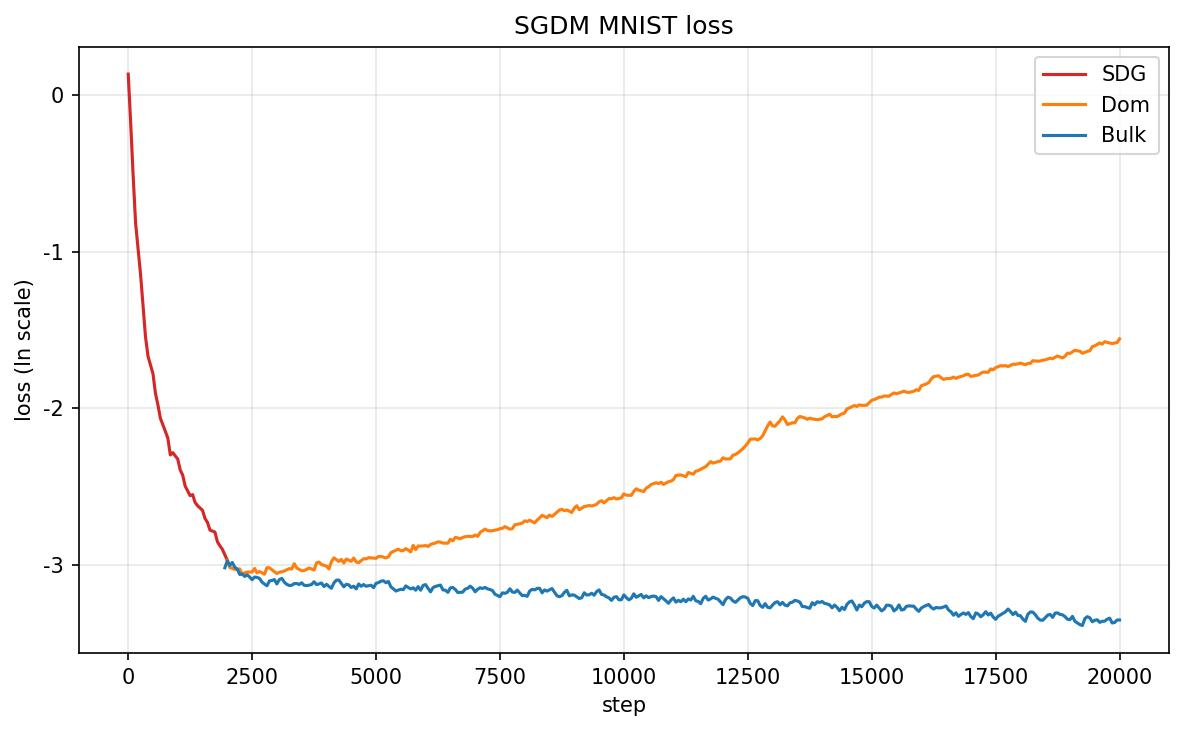
\includegraphics[width=1\linewidth]{sgdm_mnist.png}
    \caption{
    Reproduction of the MLP on MNIST-5k experiment with SGD with momentum.
    As in the SGD case, projection onto the dominant Hessian subspace prevents further loss decrease, while projection onto the bulk subspace preserves useful training progress.
    }
    \label{fig:placeholder}
\end{figure}

\paragraph{Reproduction of the CNN on CIFAR10-5k experiment for SGD}

In addition to the MNIST-5k experiments, we also reproduced the experiment for a 3-layer CNN on the CIFAR10-5k dataset with the SGD optimizer. This experiment is important because it checks whether the observed effect persists not only for a simple MLP architecture, but also for a convolutional model on a more complex dataset.

As in the previous experiments, before the switching point the model is trained with standard SGD. After the switch, we compare two trajectories: training with the update projected onto the dominant Hessian subspace and training with the update projected onto the bulk subspace.

The obtained result again qualitatively matches the conclusions of \citet{SongDoesSGD}. After switching to the dominant projection, the loss almost stops decreasing and reaches a plateau. At the same time, the bulk projection continues to steadily decrease the loss. This shows that the effect is not specific only to MLP on MNIST: for CNN on CIFAR10-5k, the useful part of the update is also mostly preserved in the bulk subspace rather than in the top-$k$ Hessian subspace.

\begin{figure}[H]
    \centering
    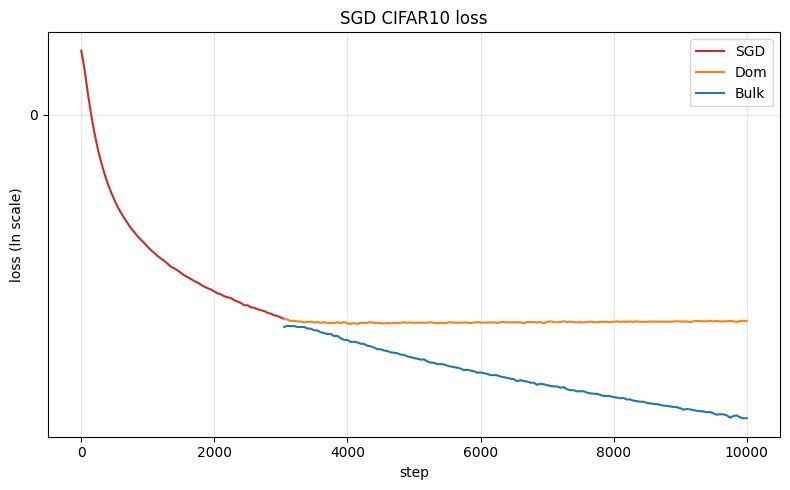
\includegraphics[width=1\linewidth]{sgd_cifar.png}
    \caption{
    Reproduction of the CNN on CIFAR10-5k experiment with SGD.
    After switching to the dominant Hessian subspace projection, the loss stops decreasing and stays almost constant.
    In contrast, projection onto the bulk subspace continues to decrease the loss, which supports the conclusion that the useful learning direction is mainly located outside the top-$k$ Hessian subspace.
    }
    \label{fig:placeholder}
\end{figure}

\paragraph{EMA alignment for Muon}

Separately, we measured the EMA of \(\chi_k\) for the Muon optimizer on the MLP on MNIST-5k task. In the protocol of \citet{SongDoesSGD}, the start of the projection phase is determined by EMA alignment: projection starts when the EMA of \(\chi_k\) exceeds the threshold \(0.95\).

In our experiment, for Muon, the EMA value does not reach the threshold \(0.95\). The mean value is approximately \(0.7856\), and the curve itself fluctuates below the required threshold. This means that for Muon, the standard switching rule from the original paper is not triggered directly: strong alignment with the top-$k$ Hessian subspace does not appear in this run.

This result is important for further work because it shows that for some optimizers, it is necessary to analyze not only the projection of the gradient, but also the geometry of the update vector itself. In particular, for Muon, it may be necessary to compare trajectories using a fixed switching step or to use other subspaces, such as a momentum-induced subspace or an adaptive/preconditioned subspace.

\begin{figure}[H]
    \centering
    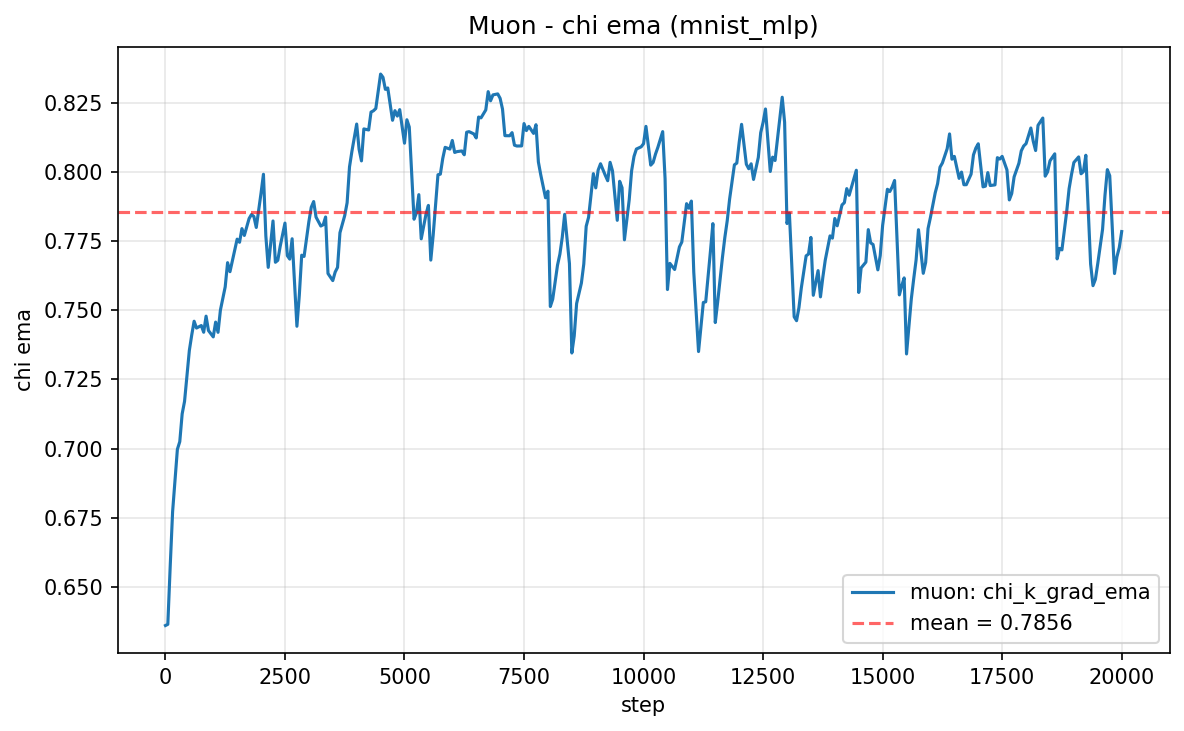
\includegraphics[width=1\linewidth]{muon_ema.png}
    \caption{
    EMA of \(\chi_k\) for Muon on MLP/MNIST-5k
    }
    \label{fig:placeholder}
\end{figure}

\section*{}
% \newpage 
\printbibliography

\appendix

\section{GitHub repository}

The source code for the project is available at:

\url{https://github.com/Oladiy2504/where_do_gradient_methods_really_happen}

\end{document}